\documentclass[conference]{IEEEtran}
% *** CITATION PACKAGES ***
\usepackage{cite}

\hyphenation{op-tical net-works semi-conduc-tor}
\bibliographystyle{vancouver}

 \usepackage[table,xcdraw]{xcolor}

\usepackage[utf8]{inputenc}
\usepackage[spanish]{babel}
\usepackage{hyperref}
\usepackage{graphicx}
\usepackage{mathtools}

\usepackage[all]{xy}

\newcommand{\sw}{plataforma}

\begin{document}
 
% paper title
% can use linebreaks \\ within to get better formatting as desired
\title{Navindoor: Plataforma de simulación para el diseño, prueba y evaluación de sistemas de localización}

\maketitle

\begin{abstract}
    En este artículo se presentará la herramienta de simulación, Navindoor. Esta es una librería para MATLAB que nos provee de las herramientas necesarias para todo el proceso de sistemas de localización.  
    \newline
\end{abstract}

\begin{IEEEkeywords}
localización en interiores, procesamiento de señales
\end{IEEEkeywords}

 
%     En este artículo se presentará la herramienta navindoor. Esta es un toolbox para MATLAB dirigido a la investigación de sistemas de posicionamiento. Navindoor contiene herramientas necesarias para el desarrollo de nuevos algoritmos, tal como el diseño del escenario, la simulación de la trayectoria o generación de señales de radiofrecuencia, inerciales, entre otras. Navindoor ha sido diseñado de forma altamenete modular en donde el ususario puede desarrolar modelos de simulación o algoritmos de posicionamiento.
\IEEEpeerreviewmaketitle

\section{Introdución}

% 1- Problema actual: experimentación en posicionamiento es costoso

Las metodologías utilizadas para los sistemas de localización son tan variadas como la diversidad de sensores existentes. Sin embargo, aunque los algoritmos sean diversos, existe una serie de pasos comunes que se deben realizar antes que desarrollar un algoritmo de posicionamiento. Estas son, la toma de medidas experimentales de señales, así como medidas de la propia trayectoria. Esta recolección de datos debe ser variada, ya que una colección en pocas casuísticas puede agregar sesgos no deseados a nuestros algoritmos. Es por ello que lo ideal es realizar pruebas en varios entornos con distintas trayectorias. Sin embargo, esto hace que el tiempo y el coste del desarrollo aumente. 

% 2- Simuladores son útiles para esta tarea
% 3- No existen demasiados actualmente y tienen algunas limitaciones: centrados en RF, no cubren todos los elementos que intervienen en un experimento

Es por ello que la simulación de señales es una tarea muy interesante. Buenos modelos de simulación pueden evitarnos pruebas experimentales antes de tener confianza completa en nuestro algortimo. Sin embargo, por ahora no existe un estandar de software donde poder desarrollar algortimos de distintas características. Los pocos simuladores que existen con este fin, suelen desarrollar en detalle alguna tecnología en concreto. Esto hace que la fusión de algoritmos o de modelos de simulación, requiera un prepoceso y el conocimiento de varios frameworks.

% 4 - - Objetivo del paper: presentar Navindoor. Introducir las principales características y diferencias con el estado del arte: framework/API Matlab, modular, incluye GUI

En este artículo se propone el software de simulación, Navindoor\footnote{\url{https://github.com/DeustoTech/navindoor-code}}. Este es un software para MATLAB, en dodne el usuario puede crear diseñar el escenario del movimiento, simular una trayectoria, geenerar señales sintéticas, además de procesar las señales generadas para crear una estimación, con ayuda de algoritmos implementados en el framework. Navindoor contiene una interfaz gráfica (GUI), que nos ayuda a generar lo antes mencionado. Sin embargo, Navindoor no solo es GUI, si no también una interfaz de lineas de comando (CLI). Esto le da la facilidad de automatizar algunas tareas. Pudiera parecer que Navindoor tambien es una estructura rígida, en donde los modelos de simulación estan anclados al framework, sin embargo, este se ha desarrollado de forma que la implementación de nuevos modelos es inmediata. Utilizando los objetos \emph{function\_handle} de MATLAB, podemos dar funciones como parámetros de entrada a los objetos de Navindoor. De esta manera desarrollar un modelo de simulación se simplifica a crear una funcion de MATLAB, con los parámetros de entrada/salida correctos.

% 5 - Estructura del resto del paper

El resto del documento se estrutura de la siguiente manera: En la sección \ref{S2}, se hará un pequeña revisión sobre los algunos simuladores, con el mismo propósito. Luego en la  sección \ref{S3}, discutiremos sobre las principales características y el diseño de Navindoor. En la sección \ref{S4} mostraremos un pequeño ejemplo de uso, y por último en la sección \ref{S5} mostraremos un pequeño resumen de los mostrado y de las siguientes desarrollos.


% ----------------------------------------------------------------------------------------------------------------------------------
% Navindoor propone una solución a este problema mediante la simulación del proceso de posicionamiento. El escenario, la trayectorias y las señales son simulados mediante modelos correspondientes. Además de permitir al usuario crear nuevos modelos si así lo quisiese. De esta forma Navindoor se convierte en un simulador muy versátil. 

% Navindoor esta diseñar para poder desarrollar tres tipos de algoritmos.
% \begin{enumerate}
%     \item \textbf{Algoritmos de simulación de trayectorias}: Los modelos de movimiento de un objetivo deberá reproducir las velocidades y aceleraciones. Este modelo puede cambiar si el objetivo es un robot o una peatón, es más el modelo de movimiento puede cambiar según el camino que tome el objetivo.
%     \item \textbf{Algoritmos de simulación de señales}: En Navindoor se contemplan dos tipos de señales, estas son las que dependen de  balizas para ser generadas y las que son solo dependientes de la trayectoria seguida (Seccion 1). Navindoor contiene modelos señales  \emph{RSS, ToF, AoA, Barometer,Magnetomer,etc.} que pueden ser modificados o creado otros a partir de ellos.
%     \item \textbf{Algoritmos de posicionamiento}: Algoritmos de posicionamiento ya concidos como los filtros de Kalman ya estan implementados en Navindoor por defecto. Y de la misma forma que en los dos puntos anteriores, la implementación de nuevos algoritmos es muy fácil.
% \end{enumerate}

% Gracias a que la herramienta contiene modelos por defecto en cada uno de sus frentes, podemos desarrollar de forma independiente a los demás modelos. 

% En este articulo, describiremos el estado del arte en materia de simuladores, además de la arquitectura de software debajo de navindoor, la funcionalidad del software en algunos ejemplos concretos y por último la dirección de los futuros desarrollos.  

 
\section{Estado del arte}\label{S2}
Los simuladores son una gran solución para mejorar el desarrollo de la sistemas de localización, es por ello que dentro la comunidad científica existen distintos intentos. A continuación mencionaremos algunos trabajos relacionados con el tema, ademas de sus principales características.

% ----------------------------------------------------


\subsection{SMILe}

SMILe \cite{Jankowski2018} es un software que propone una solución de simulación completa y unificada que ayude al desarrollo y evaluación de los métodos de localización basados en  ToF. El objetivo es proporcionar una herramienta de simulación bien definida y altamente configurable, donde se puedan evaluar varios métodos de localización. 
% pro
SMILe permite al usuario configurar un espacio, donde se pueden configurar varios factores que afectan significativamente el rendimiento general de la localización. Estos factores incluyen: despliegue de diferentes nodos, capacidades de radio, inexactitud de relojes de hardware.
% contra 
Aunque SMILe, nos provee herramientas necesarias para la comparación de algoritmos de estimación de la posición a partir de señales ToF, señales de otra índole todavía no esta implementadas. Por lo que lo hace muy potente en su especialidad y débil en otras tecnologías.
% ----------------------------------------------------

\subsection{PyLayers}

PyLayers\cite{Amiot2013} es un simulador de radio frecuencia.
% pro
El canal de radio se sintetiza mediante el uso de un método de trazado de rayos basado en gráficos, de esta forma es capaz de simular el efecto de la reflexión de las ondas.  PyLayers, esta desarrollado en python, y esta pensado para ser independientes de los algoritmos de procesamiento. 
% contra
Al igual que el simlulador anterior, aunque existe un esfuerzo por crear herramientas para todo el proceso de la localización, PyLayers se centra en las señales de radio frecuencia dejando de lado tecnologías inerciales.
% ----------------------------------------------------


\subsection{Sensor Fusion and Tracking Toolbox}

\emph{Sensor Fusion and Tracking Toolbox} \cite{Mathworks} es un toolbox desarrollado por Mathworks, que incluye algoritmos y herramientas para el diseño, simulación y análisis de sistemas que fusionan datos de múltiples sensores para sistemas de localización. Con este toolbox se puede importar y definir escenarios y trayectorias, transmitir señales y generar datos sintéticos para sensores, incluidos sensores de RF, acústicos, EO / IR y GPS / IMU. También puede evaluar la precisión y el rendimiento del sistema con puntos de referencia estándar, métricas y gráficos animados. Esta toolbox es bastante reciente, por lo que por ahora contiene pocos ejemplos, sin embargo contiene un gran potencial.  
\section{Descripción de la plataforma Navindoor}\label{S3}
% - Características generales
Navindoor ha sido desarrollado bajo el paradigma de la programación orientada a objetos. Se han definido clases para representar elementos en el diseño de sistemas de localización. La planimetría, las trayectorias o las señales son clases que contiene métodos asociados para su visualización, la extracción de datos e interacción entre ellos. Por otro lado, tenemos los algoritmos de localización y las métricas para comparar algoritmos. Estas están representadas por funciones que actúan sobre las clases antes mencionadas.
% - Funcionales
%     - Proceso de experimentación en sistemas de localización -> arquitectura modular
%     - Incluye modelos y algoritmos por defecto pero preparado para incluir nuevos
%     - Guardar/Cargar datos

Estas clases y funciones se han desarrollado en cinco módulos que siguen el proceso de experimentación en el diseño de sistemas de localización. Para tener una visión global de ello, se describirá brevemente este proceso y el módulo propuesto en cada punto:

\begin{enumerate}
    \item Obtención de la planimetría. El primer paso en la experimentación es la elección del escenario y la obtención de la planimetría de este. En Navindoor, se ha creado el módulo de planimetría con la clases necesarias para construir una planimetría de varios niveles. 
    %
    \item Generación de trayectorias. En la experimentación, se toman puntos de referencia para poder construir trayectorias a través de ellas. Esto limita la variedad de las trayectorias, sin embargo es necesario para obtener medidas precisas de la posición en cada instante. 
    %
    En Navindoor se ha creado el módulo de generación de trayectorias, dedicado a la simulación de trayectorias. Debido a que estamos en un entorno de simulación tenemos información exacta sobre la trayectoria real, generada a partir de una sucesión de puntos proporcionada por el usuario.
    %
    %
    \item Toma de medidas de señales. En la experimentación, una vez generada la trayectoria, se debe enriquecer esta con señales. El tercer módulo, llamado modulo de generación de señales, ésta dedicado a la simulación de señales sintéticas. Gracias a la simulación, podemos crear las señales después de haber sido generada la trayectoria. 
    %
    %
    \item Procesamiento de señales. Tras la toma de medidas, los algoritmos de localización se encargan de procesar las señales. El cuarto módulo de Navindoor, llamado módulo de procesamiento de medidas, provee algoritmos capaces de crear estimaciones de la trayectoria real a partir de las señales simuladas. Además de ofrecer un esquema donde nuevos algoritmos puedan ser desarrollados.
    %
    %
    \item Comparación de Algoritmos. Por último, para poder validar los algoritmos desarrollados es necesario la comparación con otros algoritmos ya consolidados. El quinto módulo de Navindoor es el módulo de validación de algoritmos, que nos provee de métodos de comparación de algoritmos proporcionados por el usuario o entre algoritmos por defecto.
\end{enumerate}
% - Técnicas
%     - Framework/API y GUI
%     - Requisitos: Matlab R2017b?
% - URL donde está disponible Navindoor
Dentro de estos módulos se encuentran repartidas las clases y funciones definidas en Navindoor. Cabe mencionar que tanto el CLI, como el GUI son compatibles en versiones de MATLAB superiores a MATLAB R2017b y se encuentran disponibles en \cite{navindoor}.

A continuación se expondrán los detalles de cada uno de los módulos.

\subsection{Creación de Planimetría}

% A- Módulo de planimetría
% - Objetivo del módulo	
El objetivo de este módulo es caracterizar el escenario donde transcurre el movimiento. Actualmente las trayectorias en Navindoor, se centran en el movimiento en interiores, por lo que se ofrece las heramientas básicas para caracterizar un edifício de varias plantas. Esta carazterización nos proveerá información sobre las restricciones de movimiento, posición de puntos de acceso, altura, etc. Esta información puede ser usada por los modelos simulación de trayectorias, señales, además de los algoritmos de localización.
% - Modelización 
%     - Diagrama de clases
%     - nodos, paredes, puertas, ascensores, escaleras, APs, plantas

Con este fin se ha definido clases de MATLAB que representarán los distintos objetos necesarios para la caracterización de un edificio. Se ha creado la clase \emph{node}, para representar un punto en el espacio tridimensional, a partir de este objeto se construyen las demás clases. Los objetos que representa las paredes del edifício, son construidos a partir de dos objetos \emph{node}. Existen tambien elementos que tiene una posición puntual, por lo que se ha creado clases que heredan las propiedades de \emph{node}. Estos son objetos \emph{stairs}, \emph{elevators}, \emph{doors}, \emph{beacons}. Los dos primeros nos idican los puntos de escape de una planta. Los objetos \emph{doors}, se definen dentro de los objetos \emph{wall}s, y permiten el paso en su entorno. Por último los objetos \emph{beacons}, representan puntos de acceso generadores de señales de radio frecuencia. Estos elementos son encapsulados en la clase \emph{level}, de modo que los objetos antes mencionados son atributos de los objetos \emph{level}. Por último se ha creado un clase, llamado \emph{building}, que en sus atributos contiene un lista de objetos \emph{levels}. Este esquema de clases se muestra en la figura \ref{fig:esquemabuilding}.

\begin{figure}[!ht]
    \centering
    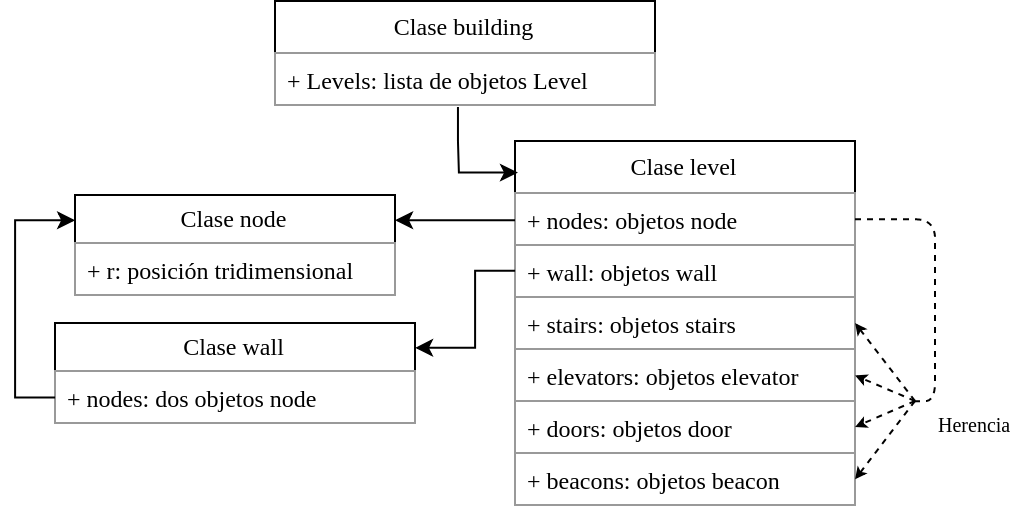
\includegraphics[width=1.05     \columnwidth]{img/Design/planimetria.png} 
    \caption[]{Esquema de la clases }
    \footnotesize
    En la imagen se intenta mostra 
    \label{fig:esquemabuilding}
\end{figure}  


% - Explicación básica del proceso de generación de planimetría:  
%     - Clicks con el ratón 
%     - mapa real como plantilla
%     - Visualización 3D
Para la creación de cada uno de estos objetos existe un constructor siguiendo las bases de la programación orientada a objetos, sin embargo la carazterización del escenario de esta forma puede ser muy tediosa. Es por ello que se ha optado en el desarrollo de una interfaz gráfica (figura \ref{fig:interfaz1}), que nos ayude en este trabajo. De esta forma se puede definir objetos \emph{nodes} con simples \emph{clicks}, y paredes uniendo objectos \emph{nodes}. 
Debido a que el proceso de creación de la planimetría puede ser tedioso, navindoor contiene una GUI capaz de generar un objeto \emph{building} (figura \ref{fig:interfaz1}). La interfaz nos permite crear los objetos antes mencionados con unos simples \emph{clicks}, además de permitir cargar una imagen de los planos reales con la que ayudarnos a construir la planimetría. Ademaś, cabe mencionar que la GUI contiene herramientas necesarias para la visualización en 3D, la modificación y eliminación de los elementos, haciendo la construcción de la planimetría intuitiva.

\begin{figure}
    \centering
    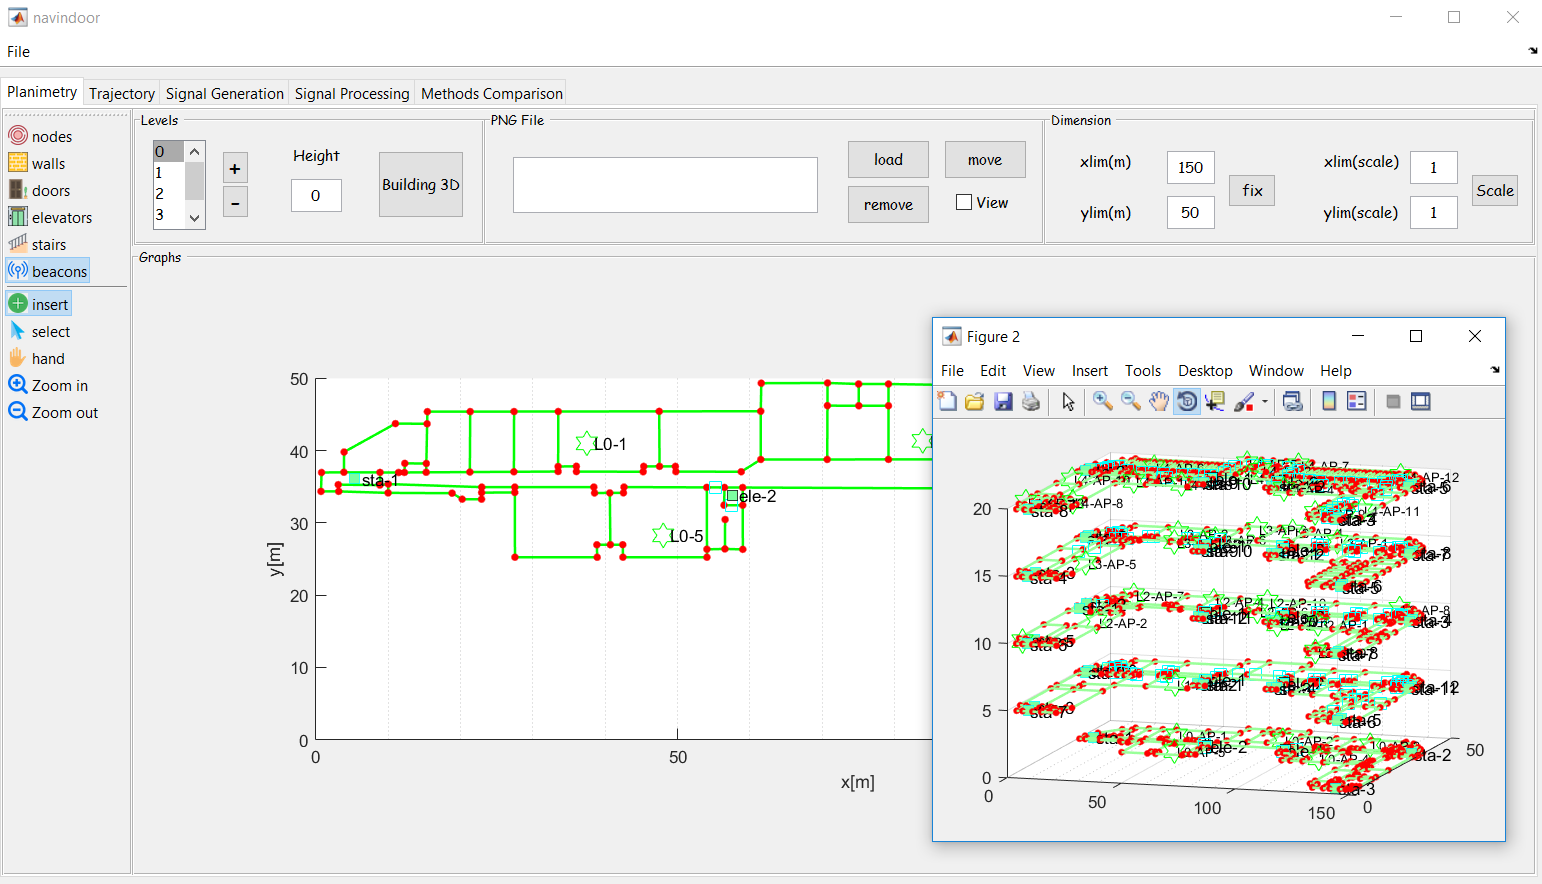
\includegraphics[width=1.05\columnwidth]{img/Design/1.PNG}
    \caption{Interfaz gráfica para el diseño de la planimetría \emph{building}.}
    \footnotesize
    En la imagen se muestra la interfaz con un edificio de cuatro plantas. La figura externa es una representación tridimensional del edificio.
    \label{fig:interfaz1}
\end{figure}

% ----------------------------------------------------------------------



\subsection{Módulo de generación de trayectorias}

% B- Módulo de generación de trayectorias
% - Objetivo del módulo	
El objetivo de este módulo es generar trayectorias dentro de la planimetría creada. La modelización de las trayectorias nos permite conseguir una vista preliminar del comportamiento de los algoritmos. Los modelos de movimiento toman importancia en este módulo, ya que de ello dependerá la similitud de los resultados obtenidos con la realidad.
% - Modelización
%       - trayectoria

En Navindoor, las trayectorias están modeladas como una sucesión de puntos dentro de la planimetría. Estos puntos definen los tramos por donde se moverá el activo. Estos se pueden definir con la ayuda de GUI, simplemente haciendo \emph{click} dentro de la planimetría, incluyendo los cambios de planta.

Un vez definida los puntos por donde pasará el activo, con ayuda de modelos de simulación se genera una sucesión de puntos más fina. Esta contiene  coordenadas de los puntos, además del instante de tiempo correspondiente. De esta forma, las velocidades y aceleraciones pueden ser obtenidas mediante diferenciación. Los modelos de generación de la trayectorias en nuestro caso están centrados en la simulación del pie de una persona, por lo que se simula medidas de los sistemas inerciales \emph{foot-mounted}. En concreto se utiliza el modelo propuesto en \cite{Zampella2011}. Además en los casos de cambios de planta se agrega un modelo de velocidad constante.

A partir de la  trayectoria del pie de la persona, se genera la trayectoria del centro de masas. Esta se usará en los casos en el que el sensor esté sobre el tronco de la persona. En la figura \ref{TrajectorySch} se muestra el proceso para la generación de un objeto trayectoria. 

Es importante notar que tanto los modelos de simulación de la trayectoria del pie, como el modelo de generación de la trayectoria del centro de masas, son parámetros opcionales. Es decir, los modelos de simulación son independientes de Navindoor, por lo que nuevos modelos pueden ser implementados creando funciones con la misma interfaz de entrada/salida que las funciones ofrecidas por defecto.

Por último, en la GUI tenemos herramientas para la generación de la trayectoria, desde la opción para crear una sucesión de puntos con \emph{clicks}, pasando por la creación de nuevos modelos, hasta la visualización de la trayectoria generada (figura \ref{fig:animation}).

\begin{figure}[ht!]
    \centering
    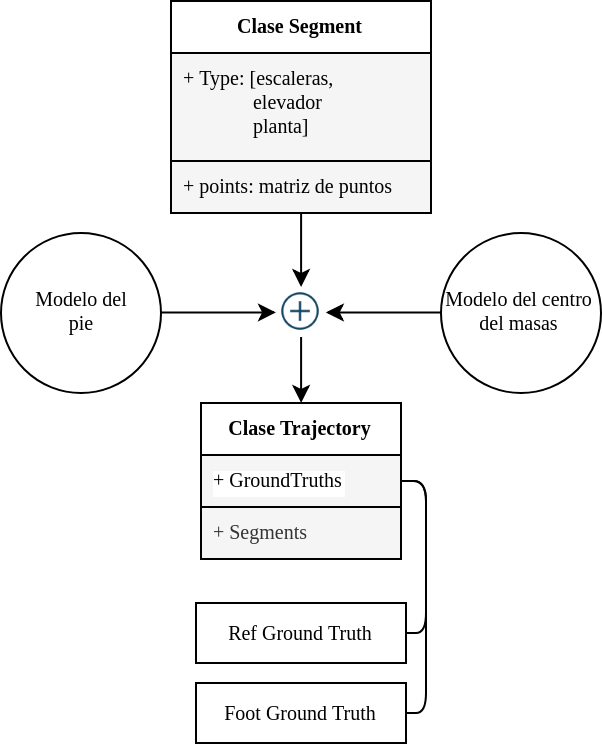
\includegraphics[width=0.75\columnwidth]{img/Design/trajectory.png}
    \caption{Proceso de construcción de una trayectoria.}
    \label{TrajectorySch}
    \footnotesize
    En este esquema se puede ver cómo el constructor de la trayectoria, genera dos objetos \emph{GroundTruths} a partir de segmentos que contienen información extraída de la planimetría. Además, es necesario un modelo que construya la trayectoria del pie de una persona a través de los segmentos y un modelo que sea capaz de crear la trayectoria del centro de masas a partir de la trayectoria del pie. El objeto \emph{Ref GroundTruth} representa la trayectoria del centro de masas, mientras que \emph{Foot GroundTruth} representa la trayectoria del pie de la persona.
\end{figure}



%       - Explicación básica del proceso de generación de trayectorias: 
%       - Selección planta
%       - Clicks con el ratón
%       - Comprobación paredes
%       - Paso a otras plantas
%   - Animación 3D

\begin{figure}
    \centering
    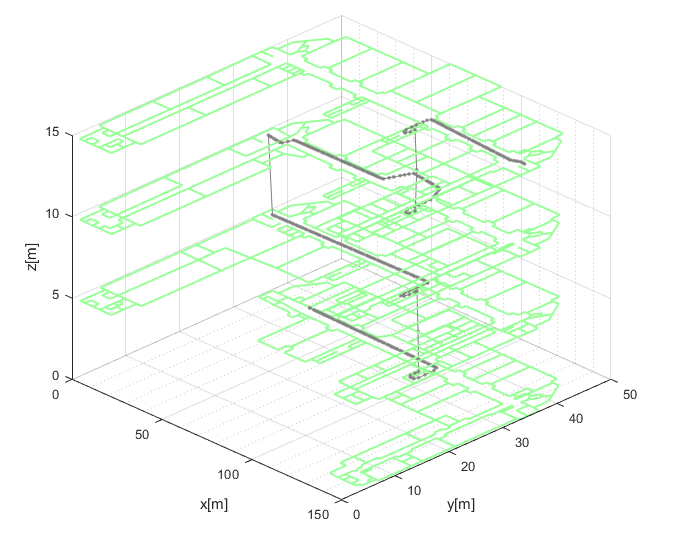
\includegraphics[width=0.8\columnwidth]{img/Design/untitled.png}
    \caption[]{Captura de una animación de una trayectoria}
    \label{fig:animation}
    \footnotesize
    Esta tiene su inicio en la planta cinco y baja usando distintas escaleras y ascensores hasta la primera planta.
\end{figure}


% ----------------------------------------------------------------------
\subsection{ Módulo de generación de señales}

% C- Módulo de generación de medidas asociadas a una trayectoria
% - Objetivo del módulo		
En este módulo se podrán simular distintos tipos de señales a partir de la trayectoria generada. El objetivo es generar datos que los algoritmos de localización procesarán. Al igual que en el módulo anterior, los modelos de simulación son cruciales para que el comportamiento del simulador sea fiel a la realidad. 

% - Modelización	
%     - Tipos de señales y métricas			
En Navindoor se ha creado la clase abstracta \emph{Signal} con propiedades que contiene la información de las medidas a lo largo de un periodo de tiempo. Además, se ha creado dos clases que heredan los métodos y propiedades de la clase \emph{Signal}. Estas son:
\begin{itemize}
    \item La clase \emph{BeaconBased}: Representando señales que necesitan  puntos de acceso para poder ser simuladas. 
    \item La clase \emph{BeaconFree}: Representando señales que pueden ser simuladas sin la necesidad de los puntos de acceso.
   \end{itemize}

Dentro del entorno de simulación, las diferencias entre estas clases se ven en la forma de construirlas. Mientras que la clase \emph{BeaconFree}, solo necesita la información de la trayectoria para ser definida, la clase \emph{BeaconBased} necesita los objetos \emph{beacons} definido en el módulo de la planimetría (figura \ref{schemaBB}). 

La clase \emph{BeaconBased} puede representar señales de atenuación de nivel de potencia (RSS), ángulo de llegada (AoA) y tiempo de vuelo (ToF), mientras que la clase \emph{BeaconFree} puede representar señales inerciales (aceleraciones lineales y velocidades angulares), intensidades de campo magnético y presión atmosférica. Los modelos de simulación de señales utilizados por defecto son básicos con una componente de ruido gaussiano.

% \begin{table}[ht]
%     \centering
%     \begin{tabular}{|c|c|}
%         \hline
%         {\textbf{BeaconBased}} & {\textbf{BeaconFree}}          \\ \hline
%         {Atenuación de nivel de potencia (RSS)}    & Barómetro        \\ \hline
%         {Tiempo de vuelo (ToF)}              & Acelerómetro               \\ \hline
%         {Angulo de llegada (AoA)}            & Magnetómetro             \\ \hline
%                                             & giroscopio             \\ \hline

%     \end{tabular}
%     \caption{Tipo de modelos de simulación de señales}
%     \label{tiposenales}
% \end{table}


En Navindoor se trata a los modelos como parámetros de entrada, por lo que es posible cambiarlos por modelos más complejos simplemente creando funciones con una interfaz de entrada/salida específica. En el caso de las clases \emph{BeaconBased}, los parámetros de entrada deberán ser un punto de la trayectoria y un objeto \emph{beacon}; y dar como parámetro de salida el valor de la señal. Mientras que en el caso de la clase \emph{BeaconFree}, solo se usa un punto de la trayectoria como parámetro de entrada y el valor de la señal como parámetro de salida.

%     - Diagrama de clases
\begin{figure}[ht!]
    \centering
        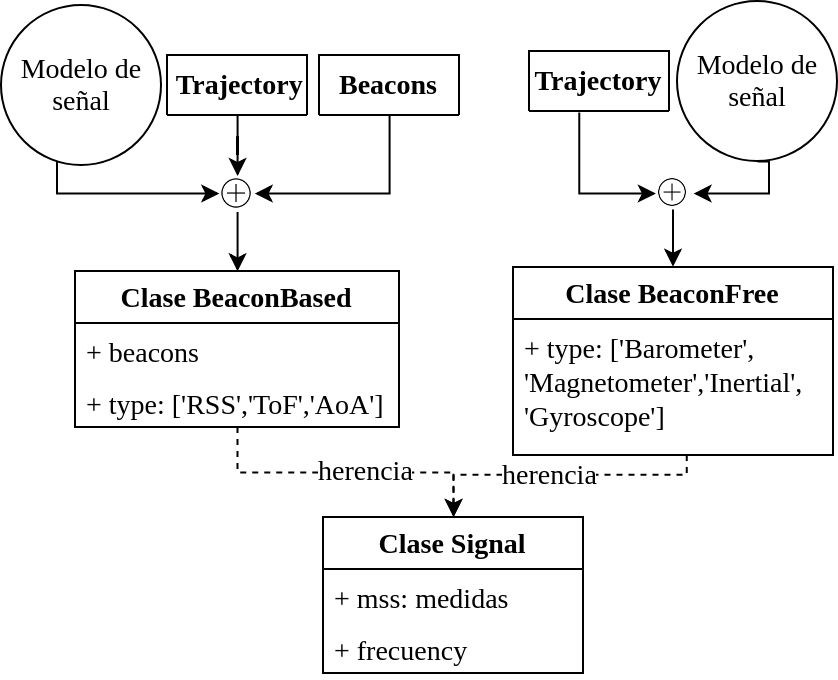
\includegraphics[width=0.85\columnwidth]{img/Design/signaldiagram.png}
        \caption{Representación de la generación de las señales.}
        \footnotesize
        Se muestra un esquema de la generación de las señales \emph{BeaconFree} y \emph{BeaconBased}. Además, también se muestra la clase \emph{Signal} de la cual heredan las propiedades donde estarán las medidas.
        \label{schemaBB}
    \end{figure} 

 

% - Explicación básica del proceso de generación de medidas asociada a una trayectoria: 
%     - Modelos de ruido: parámetros, crear modelos nuevos
%     - Visualizar señal generada
Por la parte de la GUI, en Navindoor se ha implementado un apartado para la generación de señales. En esta se muestra un listado de trayectorias previamente generadas. También se muestra un selector donde poder elegir el tipo de señal que queramos generar. Para cada uno de estos tipos nos enseña un listado de los modelos existentes. Además nos permite crear nuevos modelos a partir de una plantilla para cada tipo de señal. De esta manera dentro de la GUI podemos crear varias señales rápidamente, además de visualizar el resultado obtenido. 

% \begin{figure}[ht!]
%     \centering
%         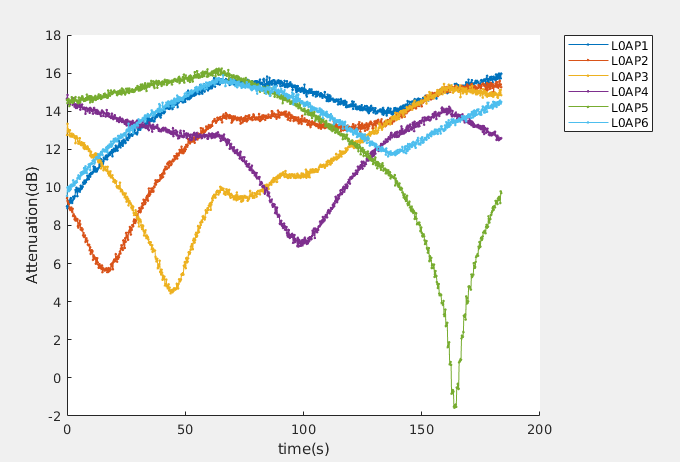
\includegraphics[width=1.0\columnwidth]{img/Design/GUIsignal.png}
%         \caption{Visualización de una señal generada en navindoor}
%         \footnotesize
%         \label{graphsBB}
%     \end{figure}


\subsection{Módulo de procesamiento de medidas}
% ----------------------------------------------------------------------
% D- Módulo de estimación de la trayectoria
% - Objetivo del módulo	
El objetivo de este módulo es proveer al usuario algoritmos básicos para la localización a partir de las señales generadas. Estos algoritmos se utilizarán como punto de partida para el diseño de nuevos. 

% - Interfaz de los algoritmos de localización
En Navindoor se encuentra implementados  el filtro de Kalman extendido (EKF)\cite{Kay:1993:FSS:151045} y el Filtro de Kalman \emph{Unscented} (UKF) \cite{UKF}. Para implementar nuevos algoritmos es necesario que estos tengan una interfaz de entrada/salida específica. Los algoritmos deberán tener tres parámetros de entrada: El objeto \emph{building}, una lista de las señales generadas en todos los instantes de tiempo y una estructura con toda la información a \emph{priori} de la trayectoria. Además deberán tener como parámetro de salida una matriz de cuatro columnas. Las tres primeras columnas indicando el espacio y la última columna el tiempo (figura \ref{format}). Navindoor se encarga de procesar esta información para crear un objeto trayectoria. De esta manera la estimación contará con las propiedades y métodos de la trayectoria real.  
\begin{figure}[ht!]
    \centering
        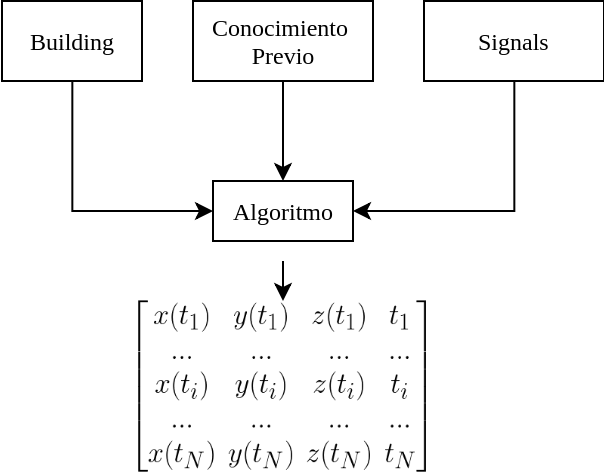
\includegraphics[width=0.725\columnwidth]{img/Design/InterfazAlgo.png}
        \caption{Interfaz de entrada/salida para los algoritmos de localización}
        \footnotesize
        Como entrada tiene tres variables, la primera representando la planimetría, la segunda representado todo el conocimiento previo sobre la trayectoria y el tercero un listado de las señales. El algoritmo devuelve una matriz $4 \times N$, siendo N el número de medidas
        \label{format}
    \end{figure}

% - Explicación básica del procesado de medidas y estimación de la trayectoria
Con respecto a la GUI, Navindoor muestra un listado de las trayectorias que han sido generadas. Para cada una de estas trayectorias podemos ver las señales disponibles. De esta manera podemos seleccionar la trayectoria y las señales que queramos procesar. Dado que los algoritmos tienen el interfaz entrada/salida antes presentado, es posible ejecutarlos con un solo \emph{click}. Navindoor, luego de ejecutar el algoritmo muestra la trayectoria real y la trayectoria estimada dentro de la planimetría cargada. Además gracias a que la estimación es un objeto trayectoria, podemos utilizar la animación utilizada en el módulo de generación de trayectorias, dando una visión a tiempo real del comportamiento de la trayectoria real frente a la trayectoria estimada.


\subsection{Comparación}

% E- Módulo de evaluación
% - Objetivo del módulo			
% - Explicación básica de la evaluación y comparación de rendimiento de los algoritmos

Por ultimo, podemos comparar los resultados de distintas ejecuciones. La diferencia de las ejecuciones puede estar el algoritmo utilizado para estimar, sin embargo también puede estar en los modelos de trayectoria, en la simulación de señales, o simplemente la frecuencia de muestreo de alguna señal. Debido a que al final del ciclo, navindoor crea trayectorias a partir de las estimaciones, las comparaciones se puede realizar entre dos estimaciones o entre la estimación y la trayectoria real. Un ejemplo de uso pordemos ve en la figura (figura \ref{fig:interfaz5}). 

\begin{figure}
    \centering
    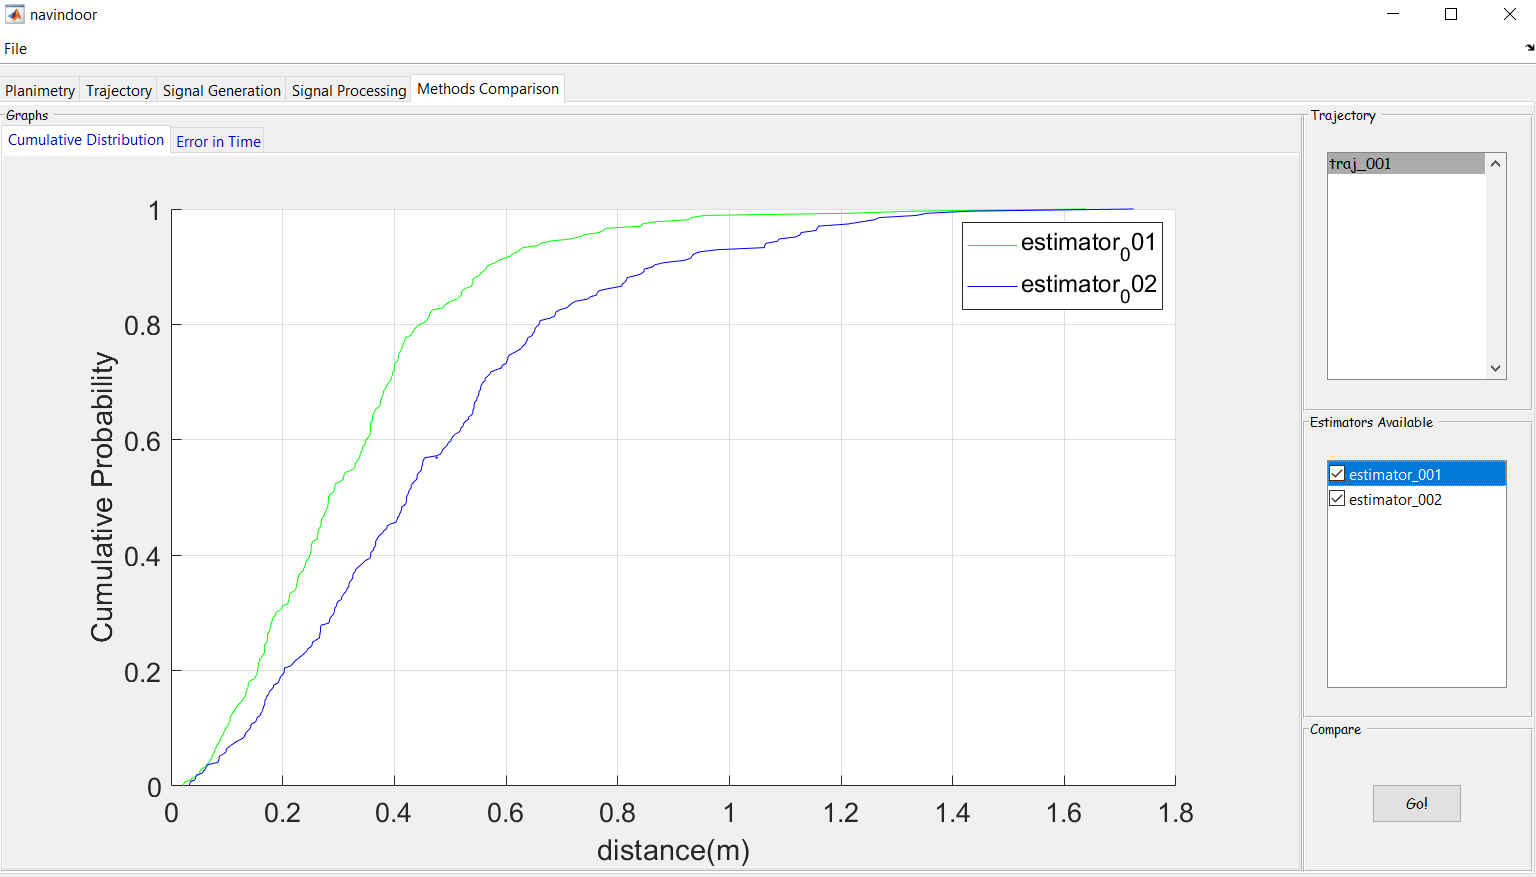
\includegraphics[width=0.8\columnwidth]{img/Design/5.PNG}
    \caption[]{Interfaz gráfica para la comparación de estimaciones.}
    \label{fig:interfaz5}
    \footnotesize 
    En este caso podemos ver el efecto de la frecuencia de muestreo en nuestras estimaciones. La estimación azul se ha realizado con una señal RSS de frecuencia 1Hz, mientras que la ver se ha realizado con una frecuencia de 5Hz.
\end{figure}


% \section{Caso de Uso}\label{S4}

% Ejemplo de utilización	
%	- Ya que tenemos hasta 6 páginas, podríamos meter 5-6 imágenes a un tamaño algo mayor, pertenecientes a un ejemplo, el cual expliquemos brevemente.


\section{Conclusiones}\label{S5}

Se han mostrado las principales características de Navindoor.  Esta plataforma ha sido desarrollada para ser escalable, donde los propios usuarios puedan contribuir con modelos de simulación de trayectorias, modelos de señales y con algoritmos de localización. Aunque en este momento los modelos implementados son básicos, su estructura modular es capaz de integrar modelos complejos.
%  

A continuación mencionaremos los futuros desarrollos en la plataforma Navindoor.

Con respecto al módulo de la planimetría, es importante notar que la clase \emph{building} es una abstracción de un edificio, por lo que la traslación a otros formatos como \emph{XML} o \emph{JSON} es inmediata. Este desarrollo permitirá comunicaciones con plataformas como \emph{Open Street Maps}, permitiendo el uso de señales \emph{GNSS}, además de la fusión de tecnologías de localización en interiores con tecnologías de localización globales.
%

En cuanto a la simulación de trayectorias, se han implementado modelos de simulación de personas. Sin embargo esto puede generalizarse a otros tipos de activos como pueden ser los drones, robots, etc. Gracias a la fácil implementación de modelos, Navindoor es una plataforma muy versátil.

Por parte de la simulación de señales, gracias a las APIs de MATLAB para otros lenguajes de programación, es posible la integración de otros simuladores en distintos lenguajes. Simuladores como los presentados en la sección \ref{S2}, pueden ser integrados.

% 
Por último, se agregarán nuevas métricas para la comparación de trayectorias, siguiendo la misma filosofía modular tomada en los modelos de simulación y los algoritmos. De esta forma, podremos crear métricas de localización personalizadas e independientes a la plataforma.

% 
% Navindoor es una plataforma que mejora el proceso de diseño de sistemas de localización y esta constantemente en desarrollo. Este continuará agregando funcionalidades, que estarán disponibles en \cite{navindoor}.


\addcontentsline{toc}{chapter}{\textbf{References}}
\bibliography{references.bib}

% that's all folks
\end{document}


